\documentclass[spanish,a4paper,11pt,twoside]{article}

%%%%%%%%%%%%%%%%%%%%%%%%%%%%%%%%%%%%%%%%%%%%%%%%%%%%%%%%%%%%%%%%%%%%%%%%%%%%%%%
\usepackage[dvips]{graphicx}
\usepackage[dvips]{epsfig}
\usepackage[latin1]{inputenc}
\usepackage[spanish]{babel}
\usepackage{alltt}




%%%%%%%%%%%%%%%%%%%%%%%%%%%%%%%%%%%%%%%%%%%%%%%%%%%%%%%%%%%%%%%%%%%%%%%%%%%%%%%
% Format
%%%%%%%%%%%%%%%%%%%%%%%%%%%%%%%%%%%%%%%%%%%%%%%%%%%%%%%%%%%%%%%%%%%%%%%%%%%%%%%

%%\topmargin -4 mm
%\topmargin -21 mm
%\headheight 10 mm
%\headsep 10 mm

%\textheight 229 mm
%\textheight 246 mm

%\oddsidemargin -5.4 mm
%\evensidemargin -5.4 mm
\oddsidemargin 5 mm
\evensidemargin 5 mm

%\oddsidemargin -3 mm
%\evensidemargin -3 mm

%\textwidth 17 cm
\textwidth 15 cm
%\columnsep 10 mm

\input{amssym.def}


%%%%%%%%%%%%%%%%%%%%%%%%%%%%%%%%%%%%%%%%%%%%%%%%%%%%%%%%%%%%%%%%%%%%%%%%%%%%%%%
\begin{document}
\title{El N\' umero Pi}
\author{Carolina Yanes Rivero \\
      T\' ecnicas experimentales~\footnote{Universidad de La Laguna}
      }
\date{\today}
\maketitle

%%%%%%%%%%%%%%%%%%%%%%%%%%%%%%%%%%%%%%%%%%%%%%%%%%%%%%%%%%%%%%%%%%%%%%%%%%%%%%%
\begin{abstract}
 $\pi$ (pi) es la relaci\' on entre la longitud de una circunferencia y su di\' ametro, en geometr\' ia euclidiana. 
 Es un n\' umero irracional y una de las constantes matem\' aticas m\' as importantes. Se emplea frecuentemente 
 en matem\' aticas, f\' isica e ingenier\' ia. 
\end{abstract}

%%%%%%%%%%%%%%%%%%%%%%%%%%%%%%%%%%%%%%%%%%%%%%%%%%%%%%%%%%%%%%%%%%%%%%%%%%%%%%%

\section{El nombre $\pi$}
La notaci\' on con la letra griega $\pi$ proviene de la inicial de las palabras de origen griego 'periferia' y 'per\' imetro' de un c\' irculo, notaci\' on que fue utilizada primero por William Oughtred (1574-1660) y cuyo uso fue propuesto por el matem\' atico gal\' es William Jones (1675-1749); aunque fue el matem\' atico Leonhard Euler, con su obra Introducci\' on al c\' alculo infinitesimal, de 1748, quien la populariz\' o. Fue conocida anteriormente como constante de Ludolph (en honor al matemático Ludolph van Ceulen) o como constante de Arqu\' imedes (que no se debe confundir con el n\' umero de Arqu\' imedes).
\subsection{ D\' ia de celebraci\' on del n\' umero $\pi$}
Por la forma en que se escribe en el formato usado en los Estados Unidos, el 14 de marzo (3/14) se ha convertido en una celebraci\' on no oficial para el "D\' ia Pi", deriv\' andose de la aproximaci\' on de tres d\' igitos de pi: 3,14. Normalmente la celebraci\' on se concentra a la 1:59 PM (en reconocimiento de la aproximaci\' on de seis d\' igitos: 3,14159), aunque algunas personas afirman que en realidad son las 13:59, por lo que lo correcto ser\' ia celebrar a la 1:59 AM.

  Matem\' aticos y profesores de varias escuelas alrededor del mundo organizan fiestas y reuniones en esta fecha. La fecha se celebra de maneras muy diversas: algunos grupos se re\' uen para discutir y comentar sobre la importancia de pi en sus vidas, intercambiar an\' ecdotas o teorizar c\' omo ser\' ia el mundo sin el conocimiento de pi. Otros grupos se re\' unen para ver la pel\' icula de culto, Pi, fe en el caos. Tambi\' en es frecuente comer tartas con motivos sobre $\pi$; otro juego de palabras, pues en lengua inglesa, tanto pi como pie (tarta) tienen id\' entica pronunciaci\' on.
     
\section{f\' ormulas que contienen el n\' umero $\pi$}
Euclides fue el primero en demostrar que la relaci\' on entre una circunferencia y su di\' ametro es una cantidad constante. No obstante, existen diversas definiciones del n\' umero $\pi$.
\subsection{Geometr\' ia}
   Veamos distintos tipos de \' areas donde el n\' umero $\pi$ es fundamental para hallarlas.
   \begin{itemize}
  \item \' Area de secciones c\' onicas
    \begin{itemize}
      \item \' Area del c\' irculo de radio r: A = $\pi$*r*r
      \item \' Area interior de la elipse con semiejes a y b: A = $\pi$*a*b
    \end{itemize}
    \begin{itemize}
  \item \' Areas de cuerpos de revoluci\' on
    \begin{itemize}
      \item \' Area del cilindro: 2*$\pi$*r*(r+h)
      \item \' Area del cono: $\pi$*r*r + $\pi$*r*g
      \item \' Area de la esfera: 4*$\pi$*r*r 
    \end{itemize}
    \end{itemize}
    \end{itemize}
    
    
%%%%%%%%%%%%%%%%%%%%%%%%%%%%%%%%%%%%%%%%%%%%%%%%%%%%%%%%%%%%%%%%%%%%%%%%%%%%%%%



\begin{figure}[!th]
\begin{center}
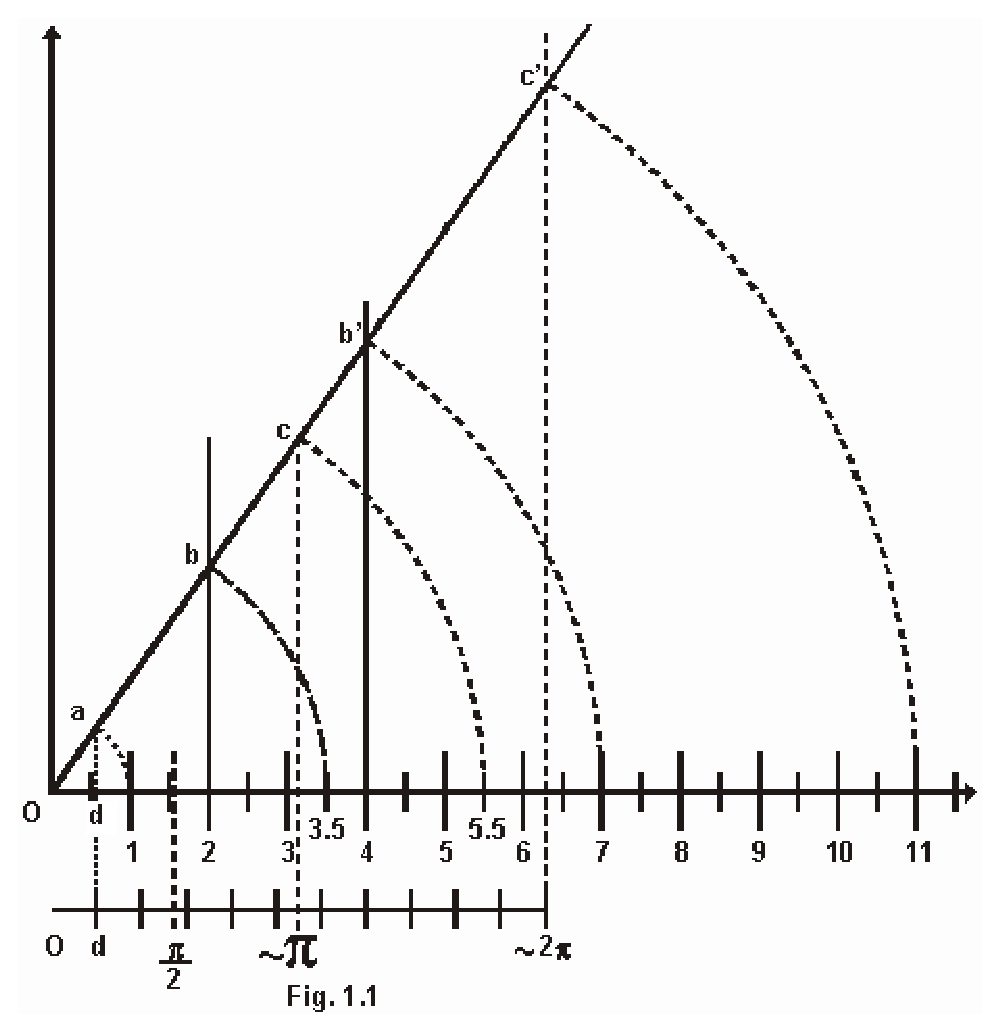
\includegraphics[width=0.25\textwidth]{fugura1.eps}
\caption{M\' etodo de Kochanski}
\label{Kochanski}
\end{center}
\end{figure}


%%%%%%%%%%%%%%%%%%%%%%%%%%%%%%%%%%%%%%%%%%%%%%%%%%%%%%%%%%%%%%%%%%%%%%%%%%%%%%%


\begin{table}[!ht]
 \begin{center}
 \begin{tabular}{|l|c|c|}
 \hline
 Digito & $\pi$ & BCD \\ \hline
  1     &  3    & 0 0 1 1 \\ \hline
  2     &  1    & 0 0 0 1 \\ \hline
  3     &  4    & 0 1 0 0 \\ \hline
  4     &  1    & 0 0 0 1 \\ \hline
  5     &  5    & 0 1 0 1 \\ \hline
  6     &  9    & 1 0 0 1 \\ \hline
  7     &  2    & 0 0 1 0 \\ \hline
  8     &  6    & 0 1 1 0 \\ \hline
  9     &  5    & 0 1 0 1 \\ \hline
  10    &  4    & 0 1 0 0 \\ \hline
 \end{tabular}
 \end{center}
 \caption{Tabla del numero Pi}
 \label{tab}
 \end{table}




%%%%%%%%%%%%%%%%%%%%%%%%%%%%%%%%%%%%%%%%%%%%%%%%%%%%%%%%%%%%%%%%%%%%%%%%%%%%%%%
\addcontentsline{toc}{chapter}{Bibliograf\' ia}
\bibliographystyle{plain}


\bibliography{bib/references}
\nocite{*}

%%%%%%%%%%%%%%%%%%%%%%%%%%%%%%%%%%%%%%%%%%%%%%%%%%%%%%%%%%%%%%%%%%%%%%%%%%%%%%%

\end{document}
